\documentclass[10pt, a4paper]{article}
\usepackage[utf8]{inputenc}
\usepackage[spanish]{babel}

\usepackage{varwidth}
\usepackage{graphicx}
\usepackage{eurosym} % para el euro

\usepackage[T1]{fontenc} % Use 8-bit encoding that has 256 glyphs


\usepackage[hmarginratio=1:1,top=32mm,columnsep=20pt]{geometry} % Document margins
\usepackage[hang, small,labelfont=bf,up,textfont=it,up]{caption} % Custom captions under/above floats in tables or figures

\usepackage{float} % Required for tables and figures in the multi-column environment - they need to be placed in specific locations with the [H] (e.g. \begin{table}[H])

\usepackage{hyperref} % For hyperlinks in the PDF


\usepackage{amsmath,amssymb}


\usepackage{titlesec} % Allows customization of titles
\renewcommand\thesection{} % Roman numerals for the sections
\renewcommand\thesubsection{\alph{subsection}} % Roman numerals for subsections
\titleformat{\section}[block]{\large\scshape\centering}{\thesection}{1em}{} % Change the look of the section titles
\titleformat{\subsection}[block]{\large}{\thesubsection.}{1em}{} % Change the look of the section titles

\usepackage{fancyhdr} % Headers and footers
\pagestyle{fancy} % All pages have headers and footers
\fancyhead{} % Blank out the default header
\fancyfoot{} % Blank out the default footer
\fancyhead[C]{Sergio García Prado $\bullet$ Mayo 2016 $\bullet$ Modelos para la Toma de Decisiones $\bullet$ Tarea 2} % Custom header text
\fancyfoot[RO,LE]{\thepage} % Custom footer text

%----------------------------------------------------------------------------------------
%	TITLE SECTION
%----------------------------------------------------------------------------------------

\title{\vspace{-15mm}\fontsize{24pt}{10pt}\selectfont\textbf{Modelos para la Toma de Decisiones: Tarea 2}} % Article title

\author{
\large
\textsc{Sergio García Prado}\\[2mm] % Your name
\normalsize Universidad de Valladolid \\ % Your institution
\vspace{-5mm}
}
\date{}

%----------------------------------------------------------------------------------------

\begin{document}

	\maketitle % Insert title

	\thispagestyle{fancy} % All pages have headers and footers

%----------------------------------------------------------------------------------------
%	TEXT
%----------------------------------------------------------------------------------------

    \section{Ejercicio 1}

        \begin{figure}[H]
        \centering
            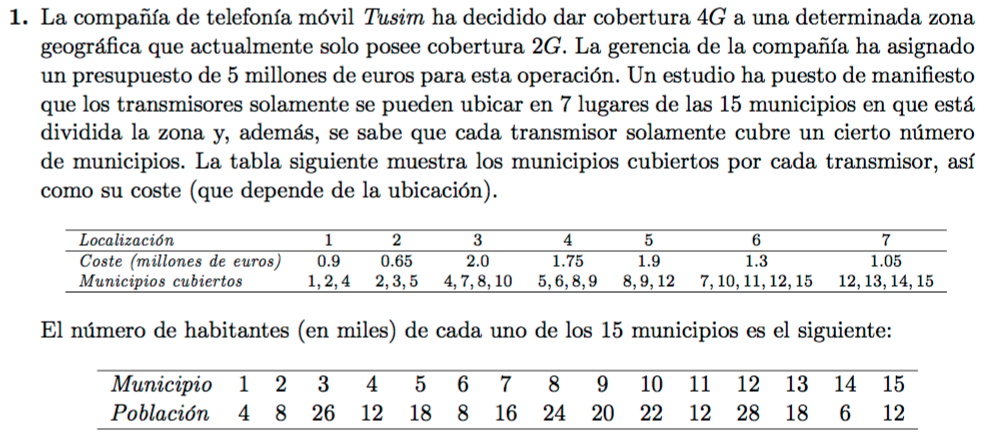
\includegraphics[width=\textwidth]{res/exercise-1.png}
        \end{figure}


		\subsection{Formular un modelo de PLE para determinar dónde se deben construir los transmisores para cubrir la mayor población con el límite del presupuesto de 5 millones de euros.}

			\paragraph{}

		\subsection{?`Cuántos transmisores se deben construir y en qué lugares? ?`Cuál es el tamaño de la población cubierto por esos transmisores? ?`Y el coste de la operación? ?`Existen municipios sin cubrir por esos transmisores?. Justificar las respuestas.}

			\paragraph{}


	\section{Ejercicio 2}

        \begin{figure}[H]
        \centering
            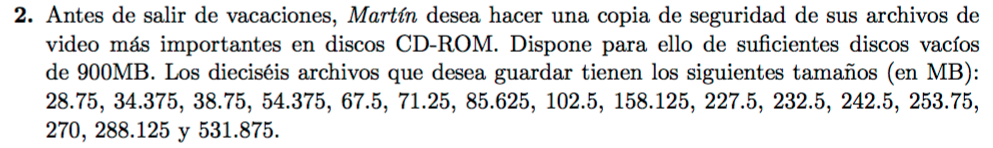
\includegraphics[width=\textwidth]{res/exercise-2.png}
        \end{figure}


		\subsection{Suponiendo que Martín no tiene ningún programa para comprimir los archivos, formular un modelo de PLE para determinar cómo se deben distribuir los archivos con el fin de reducir al mínimo el número de discos CD-ROM que debe utilizar.}

			\paragraph{}

		\subsection{?`Cuántos CD debe utilizar y qué archivos debe ubicar en cada uno de ellos? Justificar la respuesta.}

			\paragraph{}


	\section{Ejercicio 3}

        \begin{figure}[H]
        \centering
            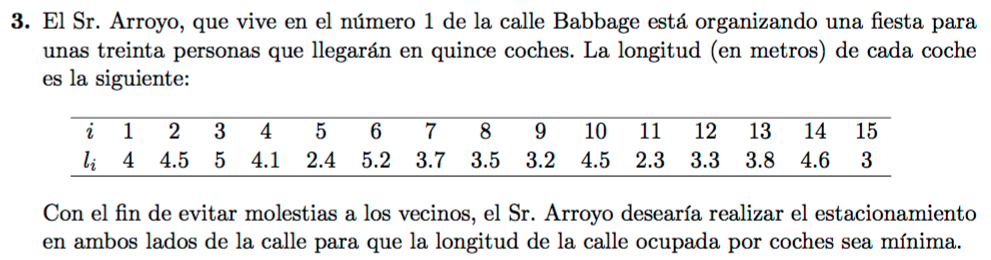
\includegraphics[width=\textwidth]{res/exercise-3.png}
        \end{figure}


		\subsection{Formular un modelo PLE para resolver el problema.}

			\paragraph{}

		\subsection{Indicar la solución óptima del modelo planteado en el apartado anterior.}

			\paragraph{}

		\subsection{Supongamos ahora que en uno de los lados de la calle no deben ocupar más de 15 metros. Formular y resolver este nuevo problema.}

			\paragraph{}
\end{document}
